\documentclass[11pt,a4paper,titlepage]{article}
\usepackage[latin1,utf8]{inputenc}
\usepackage[portuguese]{babel}
\usepackage[T1]{fontenc}
\usepackage{amsmath}
\usepackage{amsfonts}
\usepackage{amssymb}
\usepackage{graphicx}
\usepackage{titlepic}
\usepackage{geometry}
\usepackage{multicol}
\usepackage{eurosym}
\usepackage[table, xcdraw, usenames, dsipsnames]{xcolor}
\usepackage{booktabs}
\geometry{top=2cm, bottom=2cm}
\title{Seguros de Saúde\\Produção de Documentos Técnicos}
\author{Miguel Figueiredo Carmona Simões Nunes\\fc56338\quad TP19\\fc56338@alunos.fc.ul.pt\\Licenciatura em Engenharia Informática}
\date{}
\titlepic{
\includegraphics[scale=2]{SeguroSaude.jpg}}
\begin{document}
\maketitle
\tableofcontents
\pagenumbering{Roman}
\setcounter{page}{1}
\newpage
\pagenumbering{arabic}
\section{Introdução}
Um seguro de saúde protege o titular, e eventualmente, caso contratado, a sua família, de intervenções na área da saúde servindo de alternativa ao Serviço Nacional de Saúde. Através do pagamento de um prémio mensal, o segurado terá a comparticipação de parte ou da totalidade das suas despesas de saúde, sendo o valor do respetivo prémio dependente do tipo e da dimensão das coberturas. Existem três tipos distintos de seguros de saúde:
\begin{description}
\item[Reembolso] Depois de ter feito o seu tratamento e depois de o pagar, a seguradora reembolsa-lhe uma percentagem da despesa que suportou;
\item[Co-pagamento] O cliente usufruiu de um preçário fixo por tratamento ou por consulta, dentro de uma rede de prestadores. Neste caso, haverá lugar ao pagamento de um género de taxa moderadora (franquia) que depende do seguro e dos acordos;
\item[Misto] Existe a possibilidade de fazer um misto entre as duas modalidades acima identificadas, dependendo da sua conveniência e opção.
\end{description}
Aqui estão algumas vantagens e desvantagens dos seguros de saúde (dependentemente do seguro):
\begin{center}
\begin{multicols}{2}
\textbf{Vantagens}\\
\begin{itemize}
\item Liberdade de escolha do hospital/médico pelo qual quer ser atendido;
\item Tempos de espera muito menores;
\item Benefícios extra (apoio domiciliário, medicamentos ao domicilio, opinião internacional).
\end{itemize}
\quad \\ \quad \\ \quad \\ \quad \\
\textbf{Desvantagens}\\
\begin{itemize}
\item Custo elevado;
\item Carência (tempo de espera entre o pagamento e quando pode usufruir dos benefícios);
\item Franquias (Pagamentos adicionais);
\item Co-pagamentos podem ser bastante significativos;
\item Algumas doenças, incluindo pré-existentes, poderão não ser incluídas.
\end{itemize}
\end{multicols}
\end{center}
\newpage
\section{Caso de Estudo}
O Sr. Nelson decidiu adquirir um seguro de saúde para o seu agregado familiar.\\
Considerando que o Sr. Nelson estima utilizar o seu seguro 70\% em horário diurno e 30\% em horário noturno, a seguradora que procurou propôs-lhe 3 seguros calculados através do seu número, 56338.
\begin{table}[htbp]
  \centering
    \begin{tabular}{|c|c|c|c|}
    \toprule
     & \multicolumn{1}{p{4.215em}|}{Seguro A} & \multicolumn{1}{p{4.215em}|}{Seguro B} & \multicolumn{1}{p{4.215em}|}{Seguro C} \\
    \midrule
    Assinatura anual & 33 & 38 & 56 \\
    \midrule
    Tarifa de ato médico diurno & 0 & 1 & 2 \\
    \midrule
    Tarifa de ato médico noturno & 4 & 4 & 7 \\
    \midrule
    Atos médicos oferecidos com a assinatura & 25 & 15 & 10 \\
    \bottomrule
    \end{tabular}
  \caption{Tabela de preços em euros}
  \label{tab1}
\end{table}
\begin{table}[htbp]
  \centering
    \begin{tabular}{|c|c|c|c|}
    \toprule
    Nº Atos Médicos Anuais & Seguro A & Seguro B & Seguro C \\
    \midrule
    10    & 33    & 38    & 56 \\
    \midrule
    20    & 33    & 47,5  & 91 \\
    \midrule
    30    & 39    & 66,5  & 126 \\
    \midrule
    40    & 51    & 85,5  & 161 \\
    \midrule
    50    & 63    & 104,5 & 196 \\
    \midrule
    60    & 75    & 123,5 & 231 \\
    \midrule
    70    & 87    & 142,5 & 266 \\
    \midrule
    80    & 99    & 161,5 & 301 \\
    \midrule
    90    & 111   & 180,5 & 336 \\
    \midrule
    100   & 123   & 199,5 & 371 \\
    \midrule
    110   & 135   & 218,5 & 406 \\
    \midrule
    120   & 147   & 237,5 & 441 \\
    \bottomrule
    \end{tabular}
  \caption{Tabela de preços em função do número de atos médicos}
  \label{tab2}
\end{table}
\begin{figure}[!h]
\centering
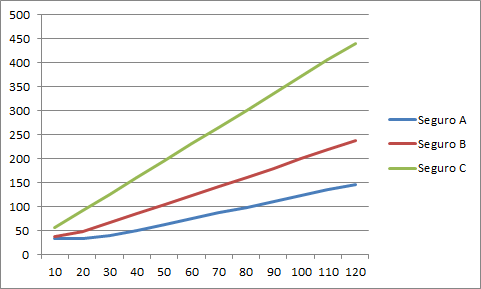
\includegraphics[scale=0.8]{Graph.png}
\caption{Representação gráfica da tabela \ref{tab2}}
\label{fig1}
\end{figure}
\newpage
\section{Conclusão}
A partir das tabelas \ref{tab1} e \ref{tab2} e da figura \ref{fig1} é fácil perceber que o Sr. Nelson deveria escolher o Seguro A pois não só são a assinatura anual e os atos médicos mais baratos, como também oferece um maior número de atos médicos grátis.
\newpage
\section{Bibliografia}
\begin{thebibliography}{9}
\bibitem{bib1} https://reorganiza.pt/o-que-e-um-seguro-de-saude/
\bibitem{bib2} https://reorganiza.pt/seguros-de-saude-vantagens-desvantagens/
\end{thebibliography}
\end{document}